\scanpage{235}

a) $\operatorname{car}k>0$, \deleted{\unsure{alors} $H^0$ fini} \inserted{et} $H^0$ \deleted{\unsure{est}} réduit à un pt; alors $G\cap H^0=\{e\}$ i.e. $\underline{\pi}_0(\varphi)$ est injectif, et du pt de vue géométrique \unsure{ensembliste} on a $\varphi=\underline{\pi}_0(\varphi)$ donc $\operatorname{Coker}\underline{\pi}_0(\varphi)$ est sans torsion

b) $\operatorname{car}k=0$, $H^0$ est un groupe \uline{vectoriel}, \deleted{\unsure{et}} donc le sous-grp fini $G\cap H^0=0$.
\margin{$G\subset H$}
D'où \deleted{\unsure{il}} on a une \unsure{s.e.} exacte
\diagram{\begin{tikzcd}
0 \arrow[r,no head] & H^0 \arrow[r] & H/G \arrow[r] & \unsure{\operatorname{Coker}\underline{\pi}_0(\varphi)} \arrow[r] \arrow[d,equal] & 0\\
 & & & H/(G+H^0) &
\end{tikzcd}}
qui \unsure{splitte} du pt de vue géométrique ensembliste (car $\unsure{H^0_{\bar{k}}|H^0}$ est divisible). Comme $H/G$ est sans torsion, il en est donc de $=$ de $\operatorname{Coker}\underline{\pi}_0(\varphi)$.

\uline{Corollaire 1} Soit $(G_n)_{n\in\unsure{\mathbf{Z}|\mathbf{N}}}$ un syst projectif de groupes \deleted{\unsure{alg.}}\inserted{comm} loc. de type fini sur le corps $k$. Supposons

\inserted{a) \deleted{\unsure{Si}} $G_0/G_0^0$ est à engendrement fini}

\inserted{\unsure{b)}} que pour tout $n$, l'hom de transition
\diagram{\begin{tikzcd}G_{n+1}\arrow[r]&G_n\end{tikzcd}}
\deleted{\unsure{ait}}\inserted{\figure{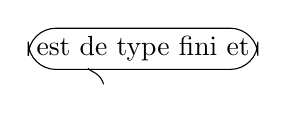
\begin{tikzpicture}[baseline=-.5ex]\node[draw,rounded corners=10pt,inner sep=3pt] at (0,0) {est de type fini et};\draw (-.7,-.25)..controls(-.65,-.3)and(-.55,-.3)..(-.5,-.45);\end{tikzpicture}}} a un noyau connexe, et un conoyau qui est géométriquement \uline{sans} torsion.

\inserted{b) pour $\forall n$, $\underline{\pi}_0(G_n)$ est à engendrement fini.}

\mspage{234}
